\documentclass[tikz,border=10pt]{standalone}
\usetikzlibrary {positioning,matrix}
\usepackage{tikzlings}
\begin{document}
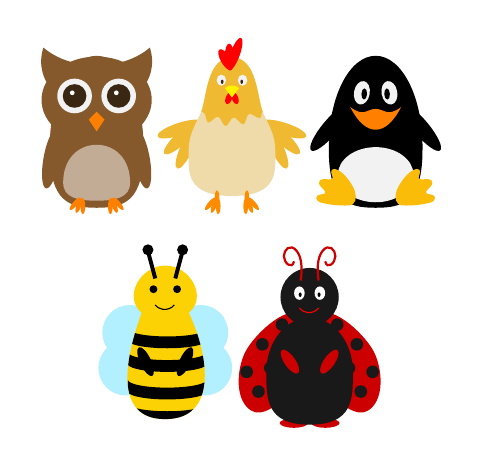
\begin{tikzpicture}
  \node (birds) [matrix] {
\owl & \chicken] & \penguin \\ };
  \node [matrix, below = 0 cm of birds] {
    \bee & \bug &  \\ };
\end{tikzpicture}

\begin{tikzpicture}
  \matrix[nodes={minimum width=6cm}] {
    \squirrel & \marmot & \moles & \sloth \\
   \pig & \koala & \coati & \panda[body=lightgray]\\
    \cat & \mouse & \sheep & \wolf\\
  };
\end{tikzpicture}
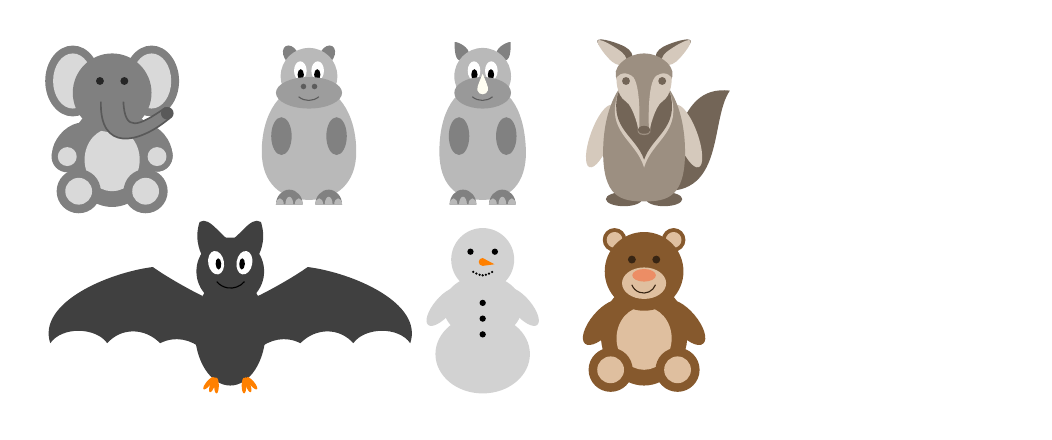
\begin{tikzpicture}
  \matrix[nodes={minimum width=6cm}] {
    \elephant \hippo[xshift=2.5cm] & \rhino & \anteater \\
    \bat[xshift=1.5cm] & \snowman[body=gray!35] & \draw (1.7,0) node{};\bear \\ };
\end{tikzpicture}
\end{document}
